\documentclass[a4paper,12pt]{book}
\usepackage[ngerman]{babel}
\usepackage[T1]{fontenc}
\usepackage[utf8]{inputenc}
\usepackage{lmodern}
\usepackage{eurosym}
\usepackage{graphicx}
\usepackage{color}
\usepackage{hyperref}
\usepackage[hypcap]{caption}
\usepackage{float}
\floatstyle{boxed} 
\restylefloat{figure}

\author{Damian Luszczymak und Karl Spies}

\date{\today}

\title{Benutzerdokumentation für die Magento Export Plattform (MEP)}

\begin{document}

\maketitle

\addcontentsline{toc}{chapter}{Inhaltsverzeichnis}
\pagenumbering{roman}
\tableofcontents
\listoffigures

\pagestyle{headings}
\pagenumbering{arabic}

\chapter{Einführung und Installation}

\section{Was ist MEP?}
\label{sec:mep}

MEP steht für "Magento Export Plattform" und soll das exportieren von
Produkte zu verschieden Preisvergleichsplattformen erleichtern. Dabei
handelt es sich um eine Neuentwicklung der Firma Flagbit GmbH \& Co. KG
und basiert technisch auf dem Import-Export Modul der Magento Community Edition.

\section{Installation}
\label{sec:install}

Es wird die Installation über die Quellen bei GitHub mittels
modman, sowie über den Magento Connect Manager (siehe Bild: 
\ref{figure:install}) im Magento-Backend unterstützt.  Nach 
erfolgreichen An- und Abmelden gibt es einen neuen Menüpunkt mit der 
Bezeichung "MEP" (siege Bild: \ref{figure:admin_menu}).

\begin{figure}
 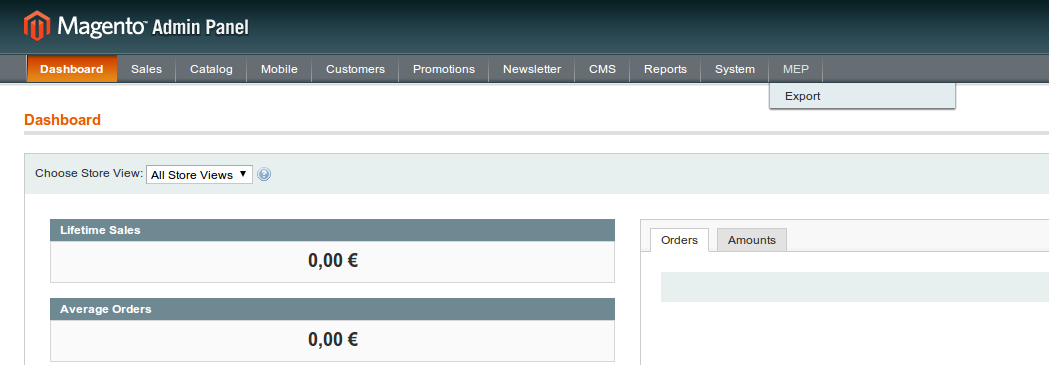
\includegraphics[width=1\textwidth]{img/bild01_1.png}
  \caption{Menüpunkt im Admin}
  \label{figure:admin_menu}
\end{figure}

\begin{figure}
 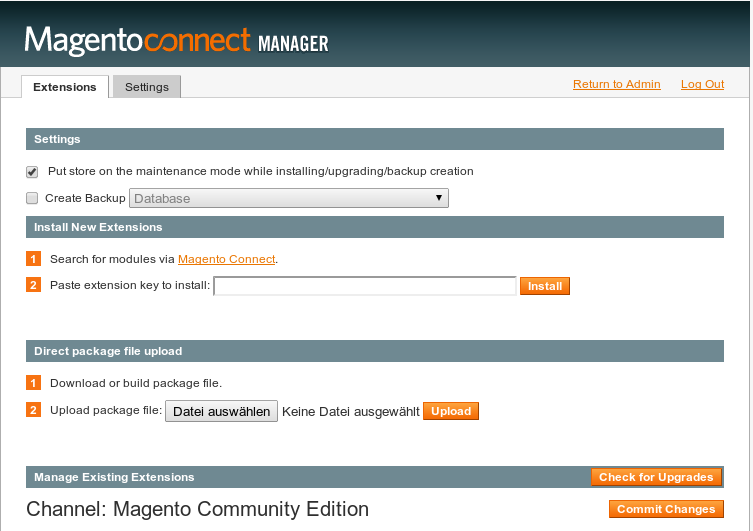
\includegraphics[width=1\textwidth]{img/bild01.png}
  \caption{Magento Connect Manager}
  \label{figure:install}
\end{figure}

\chapter{Erkärungen zum Nutzerinterface}
In MEP wird jeder neue Export als Profil angesehen. Jedes Profil ist
eine abgeschlossene Einheit. Das heißt die Profile teilen sich keine
Daten und keine Konfigurationen.

\section{Profil erstellen}
\label{sec:create}

Neue Profile werden über den Menüpunkt Export unterhalb von MEP 
erstellt. Nach dem Klick auf Export wird eine Liste der verfügbaren
Profile angezeigt. Die Tabelle zeigt alle angelegten Profile mit ihren 
ID's und Namen. Über die Spalte Action lassen sich Profile löschen 
und editieren. Die Eingabefelder oberhalb der Tabelle werden zum 
filtern und suchen verwendet.

Über "Add new" (siehe Bild: \ref{figure:new_profile}) 
können neue Profile angelegt werden. Dazu müssen folgende Daten 
bereit gestellt werden.

\begin{description}
\item[Profile Name] Der Name des Profil
\item[Status] Ein Profil kann aktiv oder inaktive sein. Dies hat
Auswirkungen beim regelmäßigen, automatischen Export.
\item[Template] In zukünftigen Versionen wird es möglich sein Vorlagen
für bestimmte Preissuchmaschine zu wählen und damit das Profil zu
erstellen
\end{description}

\begin{figure}
 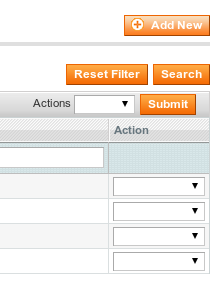
\includegraphics[width=1\textwidth]{img/bild02.png}
  \caption{Liste der Profile}
  \label{figure:profile_list}
\end{figure}

\begin{figure}
 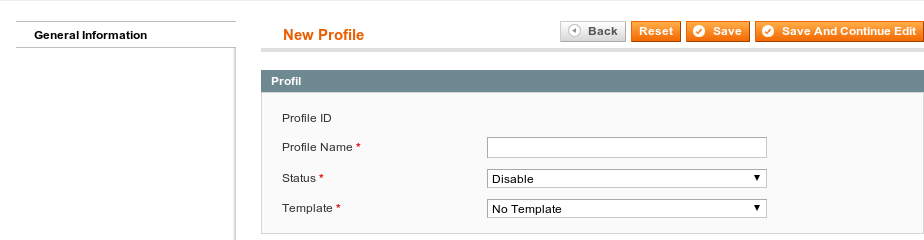
\includegraphics[width=1\textwidth]{img/bild03.png}
  \caption{Neues Profil anlegen}
  \label{figure:new_profile}
\end{figure}

Ein Klick auf "Save and Continue Edit" führt in den
Bearbeitungsmodus eines Profils. Auf der linken Seite sind die
veschiedenen Tabs zu sehen (siehe Bild: \ref{figure:new_profile_tabs}). 
Diese gruppieren die Eigenschaften des
Profils. In der rechten oberen Bereich sind die Aktionen zum
speichern (Save), speichern und weiterbearbeiten (Save and Continue
Edit), Änderungen verwerfen (Reset) und löschen (Delete) zu sehen.
Der Aktionsknopf "Run" kann zum testen des Profils verwendet werden.

\textbf{Achtung}: Bei großen Datenmengen kann dies längere Zeit in Anspruch
nehmen. Daher empfiehlt es sich den Export zum testen mittels Filter
einzuschränken. Dazu im Abschnitt \ref{sec:filter} mehr.

\begin{figure}
 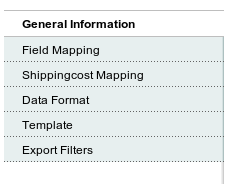
\includegraphics[width=1\textwidth]{img/bild04.png}
  \caption{Profil bearbeiten - Tabs}
  \label{figure:new_profile_tabs}
\end{figure}

\subsection{Tab Field Mapping}
\label{sec:field_mapping}

Im Tab "Field Mapping" werden die Spalten des Exports erstellt. Dazu
werden die Attribute des Produkte zugeordnet zu den Spalten im Export.
So kann zum Beispiel die SKU eines Produkte aus Magento in das Feld
"Artikelnummer" im Export kopiert werden. Dabei ist es möglich das ein
Attribut mehrfach verwendet werden kann. Zum Beispiel kann die
image\_url in das Feld "bild" und gleichzeitig auch in das Feld
"image" kopiert werden. Hierbei werden dann zwei Mappings
angelegt. Zusehen ist das im Bild:

\begin{figure}
 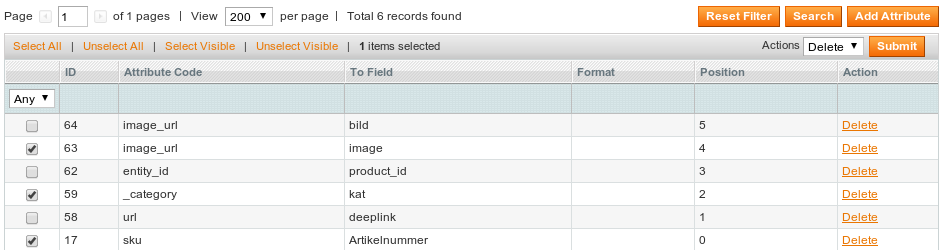
\includegraphics[width=1\textwidth]{img/bild07.png}
  \caption{Doppeltes Mapping}
  \label{figure:double_mapping}
\end{figure}

Ein Klick auf den Aktionsknopf "Add Attribute" fügt dem Profil neue 
Mappings hinzu. Es öffnet sich ein Eingabemaske in der folgende Daten 
hinterlegt werden müssen:

\begin{description}

\item[In Database] Hier werden alle Attribute nach Gruppen aufgelistet.
Das ist die Quelle für den Wert einer Zeile.

\item[To Field] Der Name der Spalte in Export. Achtung: Darf nicht mit
einer Zahl anfangen!

\item[Format] Wird bei festen Werten verwendet; siehe Spezialfälle

\item[Position] Bestimmt die Reihenfolge der Spalten im Export
\end{description}

\begin{figure}
 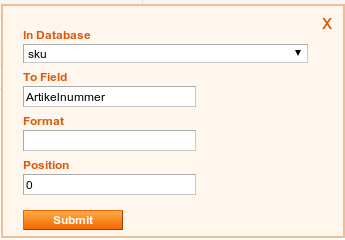
\includegraphics[width=1\textwidth]{img/bild06.png}
  \caption{Attribute hinzufügen}
  \label{figure:add_attribute}
\end{figure}

Ein erneuter Klick auf die Zeile öffnet den Dialog nochmals und es
können die Werte editiert werden. Mappings können über den "Delete"
Link am Ende einer jeden Splate in der Tabelle gelöscht werden. Wenn
mehrere Mappings gleichzeit gelöscht werden sollen, dann können diese
Markiert und über die Werkzeugleiste über der Tabelle gelöscht werden.

\begin{figure}
 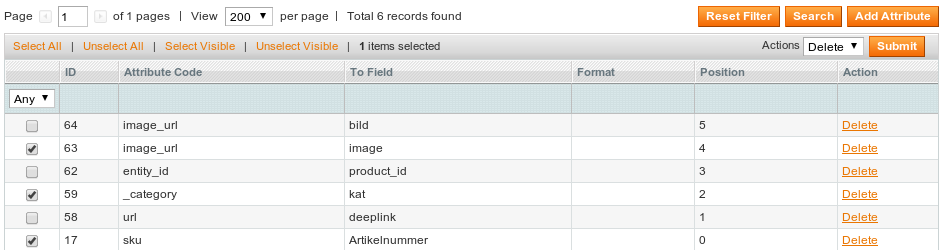
\includegraphics[width=1\textwidth]{img/bild07.png}
  \caption{Mehrere Mappings löschen}
  \label{figure:delete_massactions}
\end{figure}

\subsubsection{Spezialfälle}
\label{sec:special}
In der Liste der Attribute gibt es einige Sonderfälle und
Pseudoattribute.

\begin{description}

\item[fixed\_value\_format] In Kombination mit Format können damit feste
Werte in den Export geschrieben werden. Anwendungsfälle sind hier
Versandkosten und ähnliches

\item[url] Ist ein Deeplink auf das Produkt, enthält also keine
zusätzlichen Parameter oder Kategorien

\item[category] Hiermit wird ein Kategoriepfad ähnlich den Breadcrumbs
dem Export hinzugefügt. Wichtig ist dabei das Kategorietrennzeichen im
Tab "Dataformat"
\end{description}

\subsection{Data Format}
In diesem Tab werden alle Einstellungen für das Format des Exports
vorgenommen. Das Zielformat ist im Moment auf den Typ CSV beschränkt.
Formate wie XML und ähnliches sind für zukünftige Versionen in
Planung.

\begin{description}
\item[Value Delimiter] Der Trenner zwischen den Spalten
\item[Enclose values in] Mit welchem Zeichen sollen die Werte eines
Feldes umschlossen werden. Normalerweise wird " verwendet.
\item[Skip Headers] Soll die Kopfzeile mit den Spaltennamen ausgegeben
werden oder nicht.
\item[Name of the file] Der Name der Datei für den Export
\item[Path to export] Ich welchen Ordner soll der Export angelegt
werden. Achtung: Der Ordner muss beschreibar auf dem Server sein.
Hierbei eignen sich die Ordner media oder var
\item[Separator between categories] Welcher Trenner soll für den
Kategoriepfad eines Produktes verwendet werden.
\item[Change default locale] Hier kann die Locale Einstellung des
Servers überschrieben werden. Diese wirkt sich auf das Zahlenformat
aus. Also ob ein Punkt oder ein Komma als Dezimaltrenner verwendet
wird. Welche Werte verwendet werden können, hängt von der
Serverinstallation ab. Bitte fragen sie dies beim Hoster nach.
\end{description}


\subsubsection{Spezialfall: Use Templates}
\label{sec:templates}

Das CSV-System von MEP basiert auf der Templatesprache Twig. Aus den
Fieldmappings und den Data Format Optionen wird ein Template für den
Header und für ein Zeile des Exports generiert. Wenn die Option "Use
Templates" aktiviert wird, können die Templates direkt bearbeitet
werden. Dazu muss die Option auf Yes stehen und das Profil einmal
gespeichert werden. Erst dann steht ein zusätzlicher Tab zur Verfügung.

\textbf{Achtung}: Änderungen an den Fieldmappings müssen dann maunell
übertragen werden!

\subsection{Export Filters}
\label{sec:filter}
Jeder Profil in MEP hat die Möglichkeit die Menge der zu exportierden
Produkte einzusschränken. Dies kann nützlich sein um zum Beispiel nur
Produkte ab einem bestimmten Preis zu übermitteln oder
Speziallprodukte (Grantieverlängerungen, Versicherungem, etc.)
auszuschließen. Technisch basieren die Filter auf den
Katalogpreisregeln und lassen sich analog verwenden.

\subsubsection{Filter anlegen}
\label{sec:filter_create}
Dazu klicken sie auf das grüne Plus-Zeichen und wählen sie das
Attribut auf welches gefiltert werden soll aus. Alle fett
unterstrichenen Textelemente sind interaktiv. Sie können den Vergleich
und den Zielwert bestimmen.

Wenn sie die Option "Conditions Combination" wählen können sie
verschachtelte Bedingungen erzeugen. Zum Bespiel: "Exportiere alle
Produkte die einen Preis größer 100\euro{} haben UND einen Lagerbestand
größer 10 aber unter 50 haben. Im nachfolgenden Bild ist das einmal
dargestellt.

\begin{figure}
 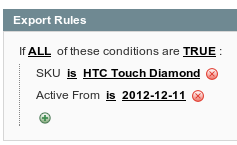
\includegraphics[width=1\textwidth]{img/bild08.png}
  \caption{Export Filter}
  \label{figure:export_filter}
\end{figure}

\subsubsection{Filter löschen}
\label{sec:filter_delete}

\textbf{Empfehlung}: Bei der Erstellung eines Profils sollten sie die Menge auf
wenige Produkte beschränken. Wenn der Export korrekt angelegt wurde,
können sie die Filter wieder entfernen.

\end{document}
